\documentclass[preprint,12pt]{elsarticle}

%% Use the option review to obtain double line spacing
%% \documentclass[preprint,review,12pt]{elsarticle}

%% Use the options 1p,twocolumn; 3p; 3p,twocolumn; 5p; or 5p,twocolumn
%% for a journal layout:
%% \documentclass[final,1p,times]{elsarticle}
%% \documentclass[final,1p,times,twocolumn]{elsarticle}
%% \documentclass[final,3p,times]{elsarticle}
%% \documentclass[final,3p,times,twocolumn]{elsarticle}
%% \documentclass[final,5p,times]{elsarticle}
%% \documentclass[final,5p,times,twocolumn]{elsarticle}

%% if you use PostScript figures in your article
%% use the graphics package for simple commands
%% \usepackage{graphics}
%% or use the graphicx package for more complicated commands
%% \usepackage{graphicx}
%% or use the epsfig package if you prefer to use the old commands
%% \usepackage{epsfig}

%% The amssymb package provides various useful mathematical symbols
\usepackage{amssymb}
%% The amsthm package provides extended theorem environments
%% \usepackage{amsthm}

%% The lineno packages adds line numbers. Start line numbering with
%% \begin{linenumbers}, end it with \end{linenumbers}. Or switch it on
%% for the whole article with \linenumbers after \end{frontmatter}.
%% \usepackage{lineno}

%% natbib.sty is loaded by default. However, natbib options can be
%% provided with \biboptions{...} command. Following options are
%% valid:

%%   round  -  round parentheses are used (default)
%%   square -  square brackets are used   [option]
%%   curly  -  curly braces are used      {option}
%%   angle  -  angle brackets are used    <option>
%%   semicolon  -  multiple citations separated by semi-colon
%%   colon  - same as semicolon, an earlier confusion
%%   comma  -  separated by comma
%%   numbers-  selects numerical citations
%%   super  -  numerical citations as superscripts
%%   sort   -  sorts multiple citations according to order in ref. list
%%   sort&compress   -  like sort, but also compresses numerical citations
%%   compress - compresses without sorting
%%
%% \biboptions{comma,round}

% \biboptions{}


\journal{Proceedings of the Royal Society B}

%%%%%%%%%%%%%%% my adding usepackages
%amsmath package provides an environment subequations
\usepackage{amsmath}

\usepackage{hyperref}

\usepackage{graphicx}



%\usepackage{showframe}

\begin{document}

\begin{frontmatter}

%% Title, authors and addresses

%% use the tnoteref command within \title for footnotes;
%% use the tnotetext command for the associated footnote;
%% use the fnref command within \author or \address for footnotes;
%% use the fntext command for the associated footnote;
%% use the corref command within \author for corresponding author footnotes;
%% use the cortext command for the associated footnote;
%% use the ead command for the email address,
%% and the form \ead[url] for the home page:
%%
%% \title{Title\tnoteref{label1}}
%% \tnotetext[label1]{}
%% \author{Name\corref{cor1}\fnref{label2}}
%% \ead{email address}
%% \ead[url]{home page}
%% \fntext[label2]{}
%% \cortext[cor1]{}
%% \address{Address\fnref{label3}}
%% \fntext[label3]{}

%Title of paper
\title{Vaccination Effect in a Many-strain Model of Influenza Drift}

%% use optional labels to link authors explicitly to addresses:
%% \author[label1,label2]{<author name>}
%% \address[label1]{<address>}
%% \address[label2]{<address>}

\author{Alvason Zhenhua Li}
\ead{alvali@fredhutch.org}

\author{Trevor Bedford}
\ead{tbedford@fredhutch.org}


\address{Vaccine and Infectious Disease Division, Fred Hutchinson Cancer Research Center, Seattle, WA 98109, USA}


\begin{abstract}
%% Text of abstract
By introducing the general vaccination strategy composing of new-born immunization(at rate \(\phi_{new}\)) and the vaccination of currently susceptible (at rate \(\phi_{pulse}\)) into the many-strain SIR epidemiological model (Gog and Grenfell 2002), a simple yet robust many-strain SIRV epidemiological model is developed for understanding the impact of vaccination at the many-strain antigenic evolution. 
\end{abstract}

\begin{keyword}
%% keywords here, in the form: keyword \sep keyword
Influenza\sep Vaccination\sep Immunity\sep Mutation
\end{keyword}

\end{frontmatter}

%% main text
\section{Introduction}
Vaccination is one of the major medical advances in fighting various virus in recent centuries. Currently, influenza vaccination is a powerful tool in the global-health control arsenal, and allows for the mass prevention of infection.
Various elements of mathematics are used throughout the vaccine development process. In this paper, we focus on the use of mathematics in influenza virus drift, understanding the impact of vaccination at the many-strain antigenic evolution. 

\section{Model}
Mathematically, based on the many-strain SIR epidemiological model (Gog and Grenfell 2002), which specifies the dynamics of large number of antigenic types with cross-immunity interaction, and introduced the general vaccination strategy composing infants (a proportion \(\phi_{new}\) of all children are assumed to be immunized) and the random vaccination of individuals in the population (at rate \(\phi_{pulse}\), although this vaccination will only affect those that are currently susceptible). We are able to developed a many-strain SIRV epidemiological model as the following:

\begin{equation}
  \label{eq:S}
  \frac{\partial S_i(x,t)}{\partial t} = \mu N(1-\phi_{new}(t)) - \mu S_i(x,t) - \phi_{pulse}(t)S_i(x,t) - \beta S_i(x,t)\sum_{y=0}^{n} I_i(y,t)\sigma(x,y)
\end{equation}

\begin{equation}
  \label{eq:I}
  \frac{\partial I_i(x,t)}{\partial t} = \beta S_i(x,t) I_i(x,t) - \mu I_i(x,t) - \nu I_i(x,t) + m I_i(x,t)
\end{equation}

\begin{equation}
  \label{eq:R}
  \frac{\partial R_i(x,t)}{\partial t} = \nu I_i(x,t) - \mu R_i(x,t) - \beta S_i(x,t) [I_i(x,t) - \sum_{y=0}^{n} I_i(y,t)\sigma(x,y)]
\end{equation}

\begin{equation}
  \label{eq:V}
  \frac{\partial V_i(x,t)}{\partial t} = \mu N \phi_{new}(t) + \phi_{pulse}(t)S_i(x,t) - \mu V_i(x,t)
\end{equation}

where the cross-immunity kernel \(\sigma(x,y)\) is an inverse form of the Monod equation:
\begin{equation}
  \label{eq:Immunity}
  \sigma(x,y) = 1 - \frac{\vert {\frac{x -y}{r}} \vert}{1 + \vert {\frac{x -y}{r}} \vert}
\end{equation}

\begin{figure}
  \centering
  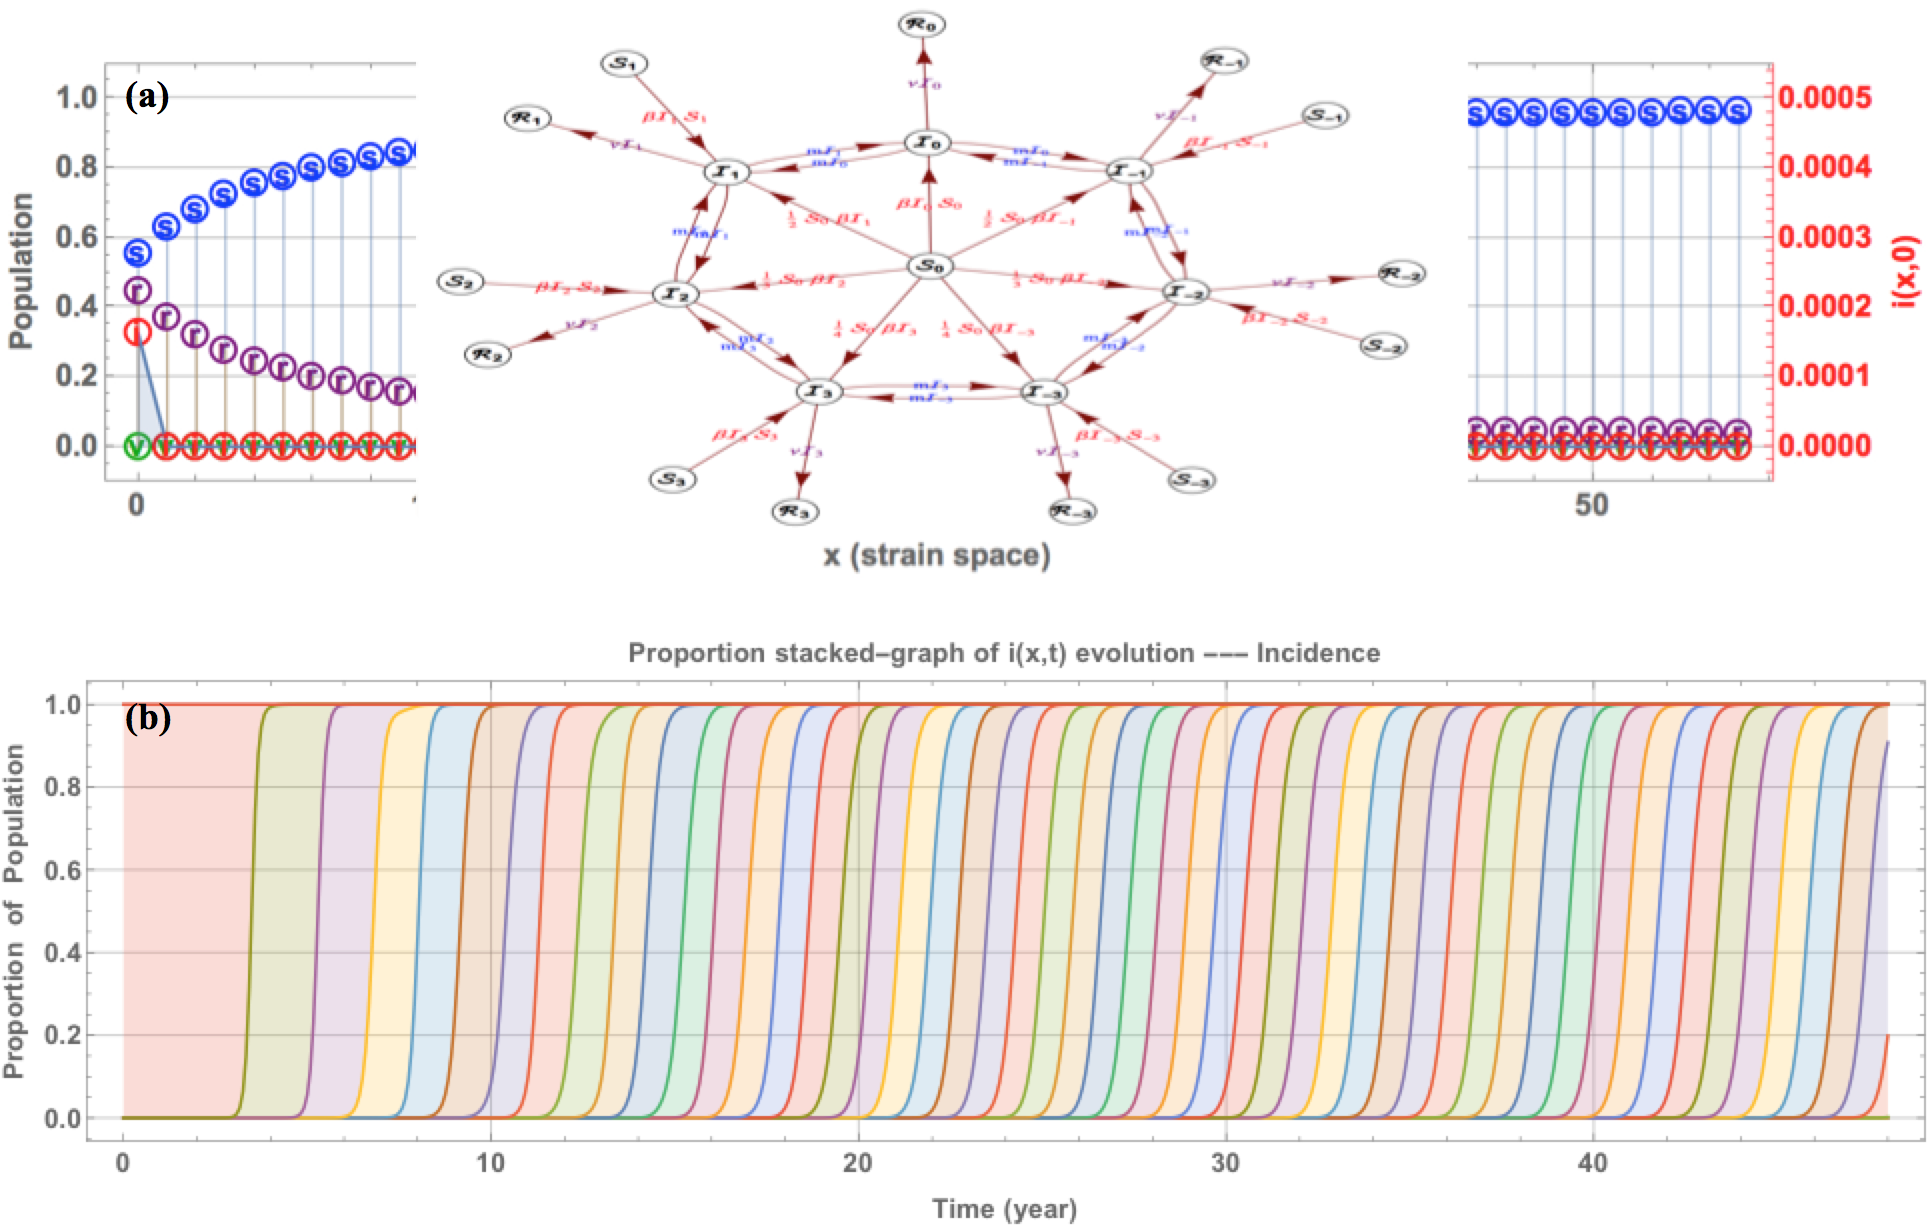
\includegraphics[width=6in,height=3in]{Diagram}
  \caption{(a) ``Temporary schematic diagram of the many-stain SIRV model" (a brand new diagram will be updated soon). (b) Proportion stacked graph indicated the building up process of steady traveling wave of influenza drift: initial single-strain-equilibrium-state is propagating into many-strain-equilibrium-state.}
\label{fig:Diagram}
\end{figure}

\section{Results}

\begin{figure}
  \centering
  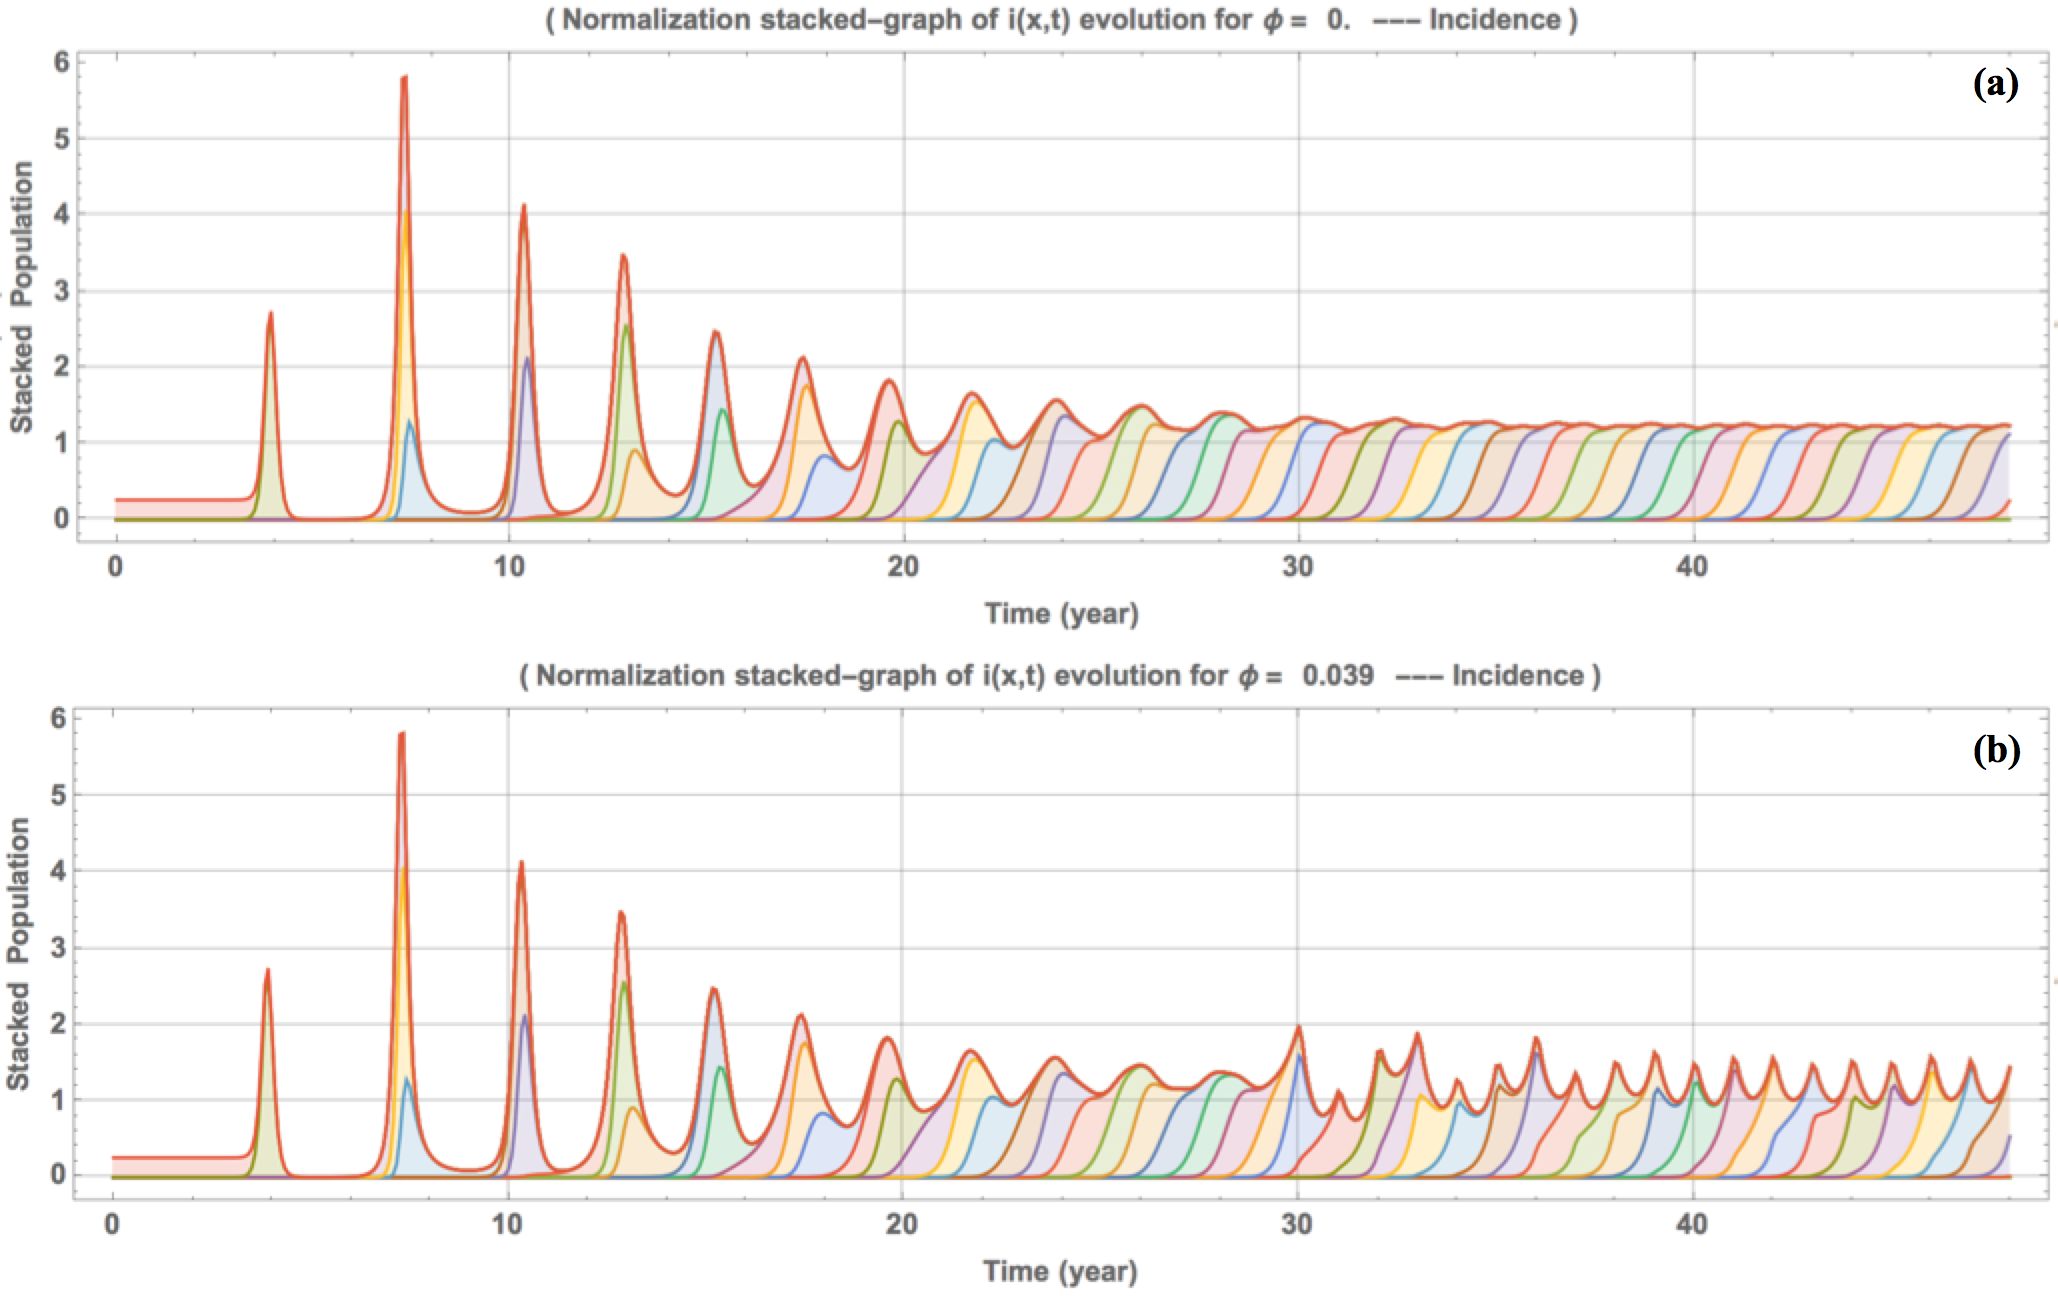
\includegraphics[width=6in,height=4in]{UnderVaccination}
  \caption{Comparison of incidence rate between non-vaccination and under-vaccination. (a) is a stain evolutionary map without vaccination (vaccination rate \(\phi\) = 0), in which a single-strain-equilibrium-state is evolving into many-strain-equilibrium-state in a half century time frame. (b) is the strain evolutionary map with 20 years vaccination: at the beginning 30 years, a single-strain-equilibrium-state is approaching into many-strain-equilibrium-state, however, starting from the 30th year, an annual vaccination strategy (vaccination rate \(\phi\) = 0.039 ) is applied. After 20 years of vaccination pressure, the evolution is evolving and approaching into vaccination-equilibrium state.}
\label{fig:UnderVaccination}
\end{figure}


\section{Analysis}
\begin{figure}
  \centering
  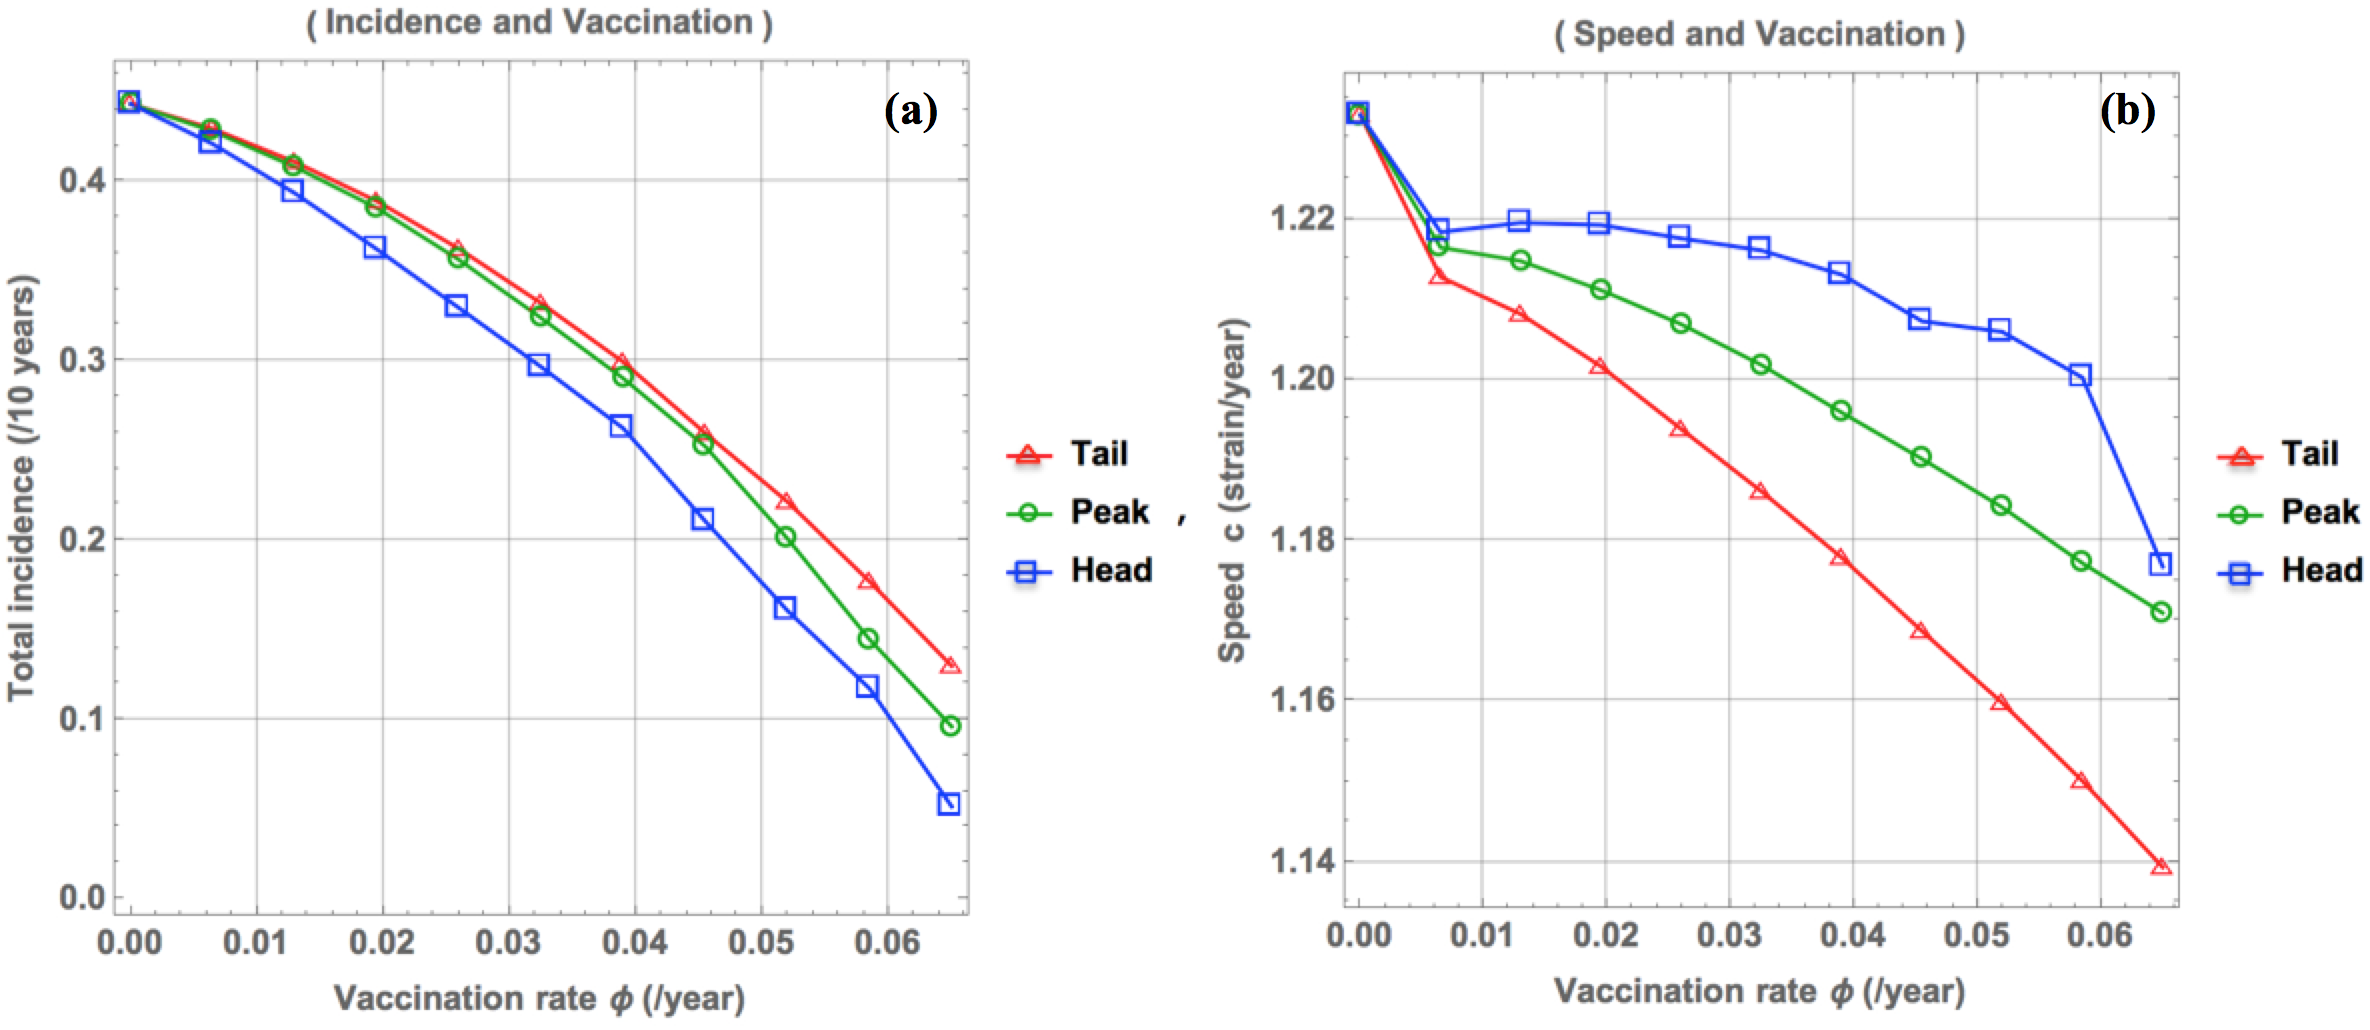
\includegraphics[width=6in,height=2.75in]{Veffect}
  \caption{Vaccination effects. (a) Total incidence rate per 10 years as a function of vaccination rate \(\phi\). (b) Speed as a function of vaccination rate \(\phi\). }
  \label{fig:Veffect}
\end{figure}



\begin{figure}
  \centering
  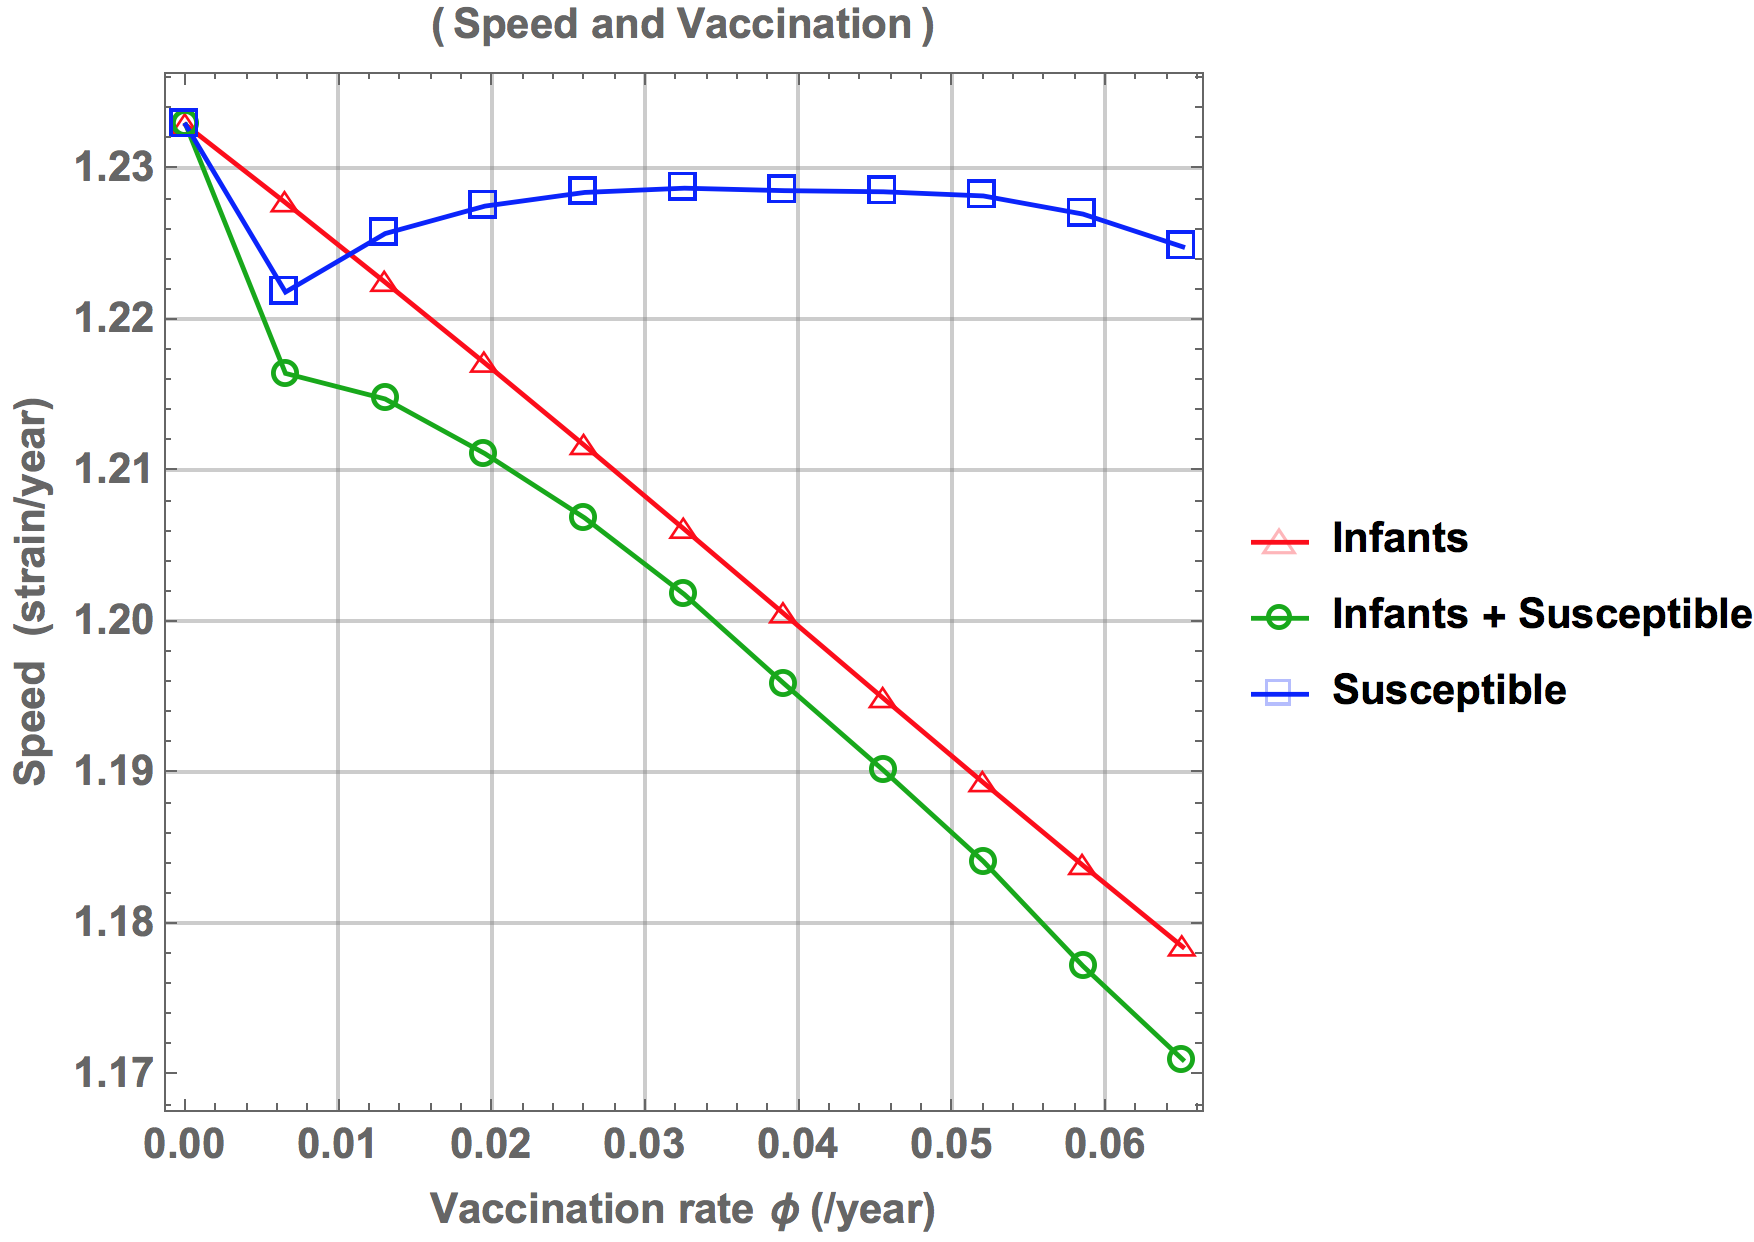
\includegraphics[width=6in,height=4in]{NewbornS}
  \caption{Contribution from two vaccination strategies. The triangle-marker red line is the strain evolutionary speed as a function of infant-vaccination-rate only, while the rectangle-marker blue line is the strain evolutionary speed as a function of susceptible-vaccination-rate only. The circle-marker green line is the composition of both vaccination strategy.}
  \label{fig:NewbornS}
\end{figure}




\section{Conclusion}
In conclusion, exact.

%% The Appendices part is started with the command \appendix;
%% appendix sections are then done as normal sections
%% \appendix

%% \section{}
%% \label{}

%% References
%%
%% Following citation commands can be used in the body text:
%% Usage of \cite is as follows:
%%   \cite{key}         ==>>  [#]
%%   \cite[chap. 2]{key} ==>> [#, chap. 2]
%%

%% References with bibTeX database:

\bibliographystyle{elsarticle-num} %with article and chapter titles,

%\bibliographystyle{model1a-num-names} %without article and chapter titles


% Create the reference section using BibTeX:
\bibliography{ReferenceMorse}

%% Authors are advised to submit their bibtex database files. They are
%% requested to list a bibtex style file in the manuscript if they do
%% not want to use elsarticle-num.bst.

%% References without bibTeX database:

% \begin{thebibliography}{00}

%% \bibitem must have the following form:
%%   \bibitem{key}...
%%

% \bibitem{}

\end{document}
